\documentclass[12pt]{book}
\usepackage[T1]{fontenc}
\usepackage{wrapfig}
\usepackage[polish]{babel}
\usepackage[utf8]{inputenc}
\usepackage{lmodern}
\usepackage{pifont}
\usepackage{amsmath}
\usepackage{cases}
\usepackage[T1]{fontenc}
\usepackage{amsthm}
\selectlanguage{polish}
\usepackage{amsmath}
\usepackage{graphicx}
\usepackage{float}
\usepackage[margin=2.5cm]{geometry}
\newcommand{\R}{\mathbb{R}}
\newcommand\addtag{\refstepcounter{equation}\tag{\theequation}}
\begin{document}
\title{Optymalizacja  systemu sygnalizacji świetlnej w 
oparciu o przepływowy model ruchu pojazdów.}
\author{Michał Lis}
\date{\today}
\maketitle
\chapter{Wprowadzenie}
\chapter{Cel pracy}
\chapter{Zakres pracy}
   
\chapter{Model sieci dróg}
\section{Drogi i skrzyżowania}
Sieć dróg przedstawia uporządkowana dwójka $G=(V,E)$, gdzie:\\ 
$V$ to zbiór skrzyżowań,\\
$E$ to zbiór dróg.\\
Droga $e \in E$ jest odcinkiem o długości $L_e$. Sieć dróg jest strukturą ograniczoną, zatem drogi mogą mieć swój początek lub koniec w punktach innych niż skrzyżowaniach (patrz rysunek \ref{fig:network}).
%\noindent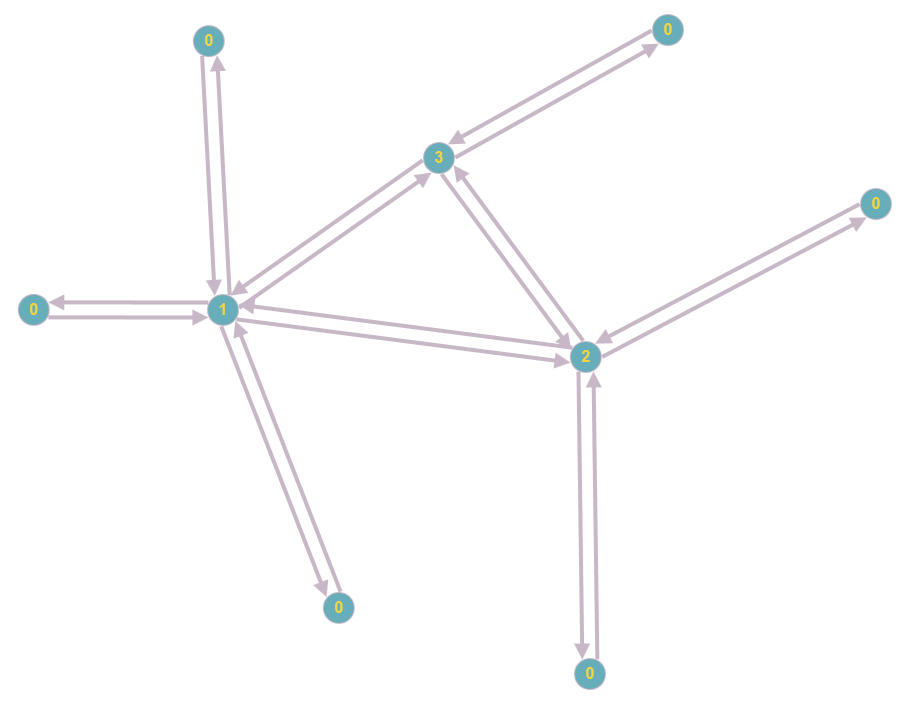
\includegraphics[width=10cm]{network} 

%\begin{wrapfigure}{R}{0.3\textwidth}
%\centering
%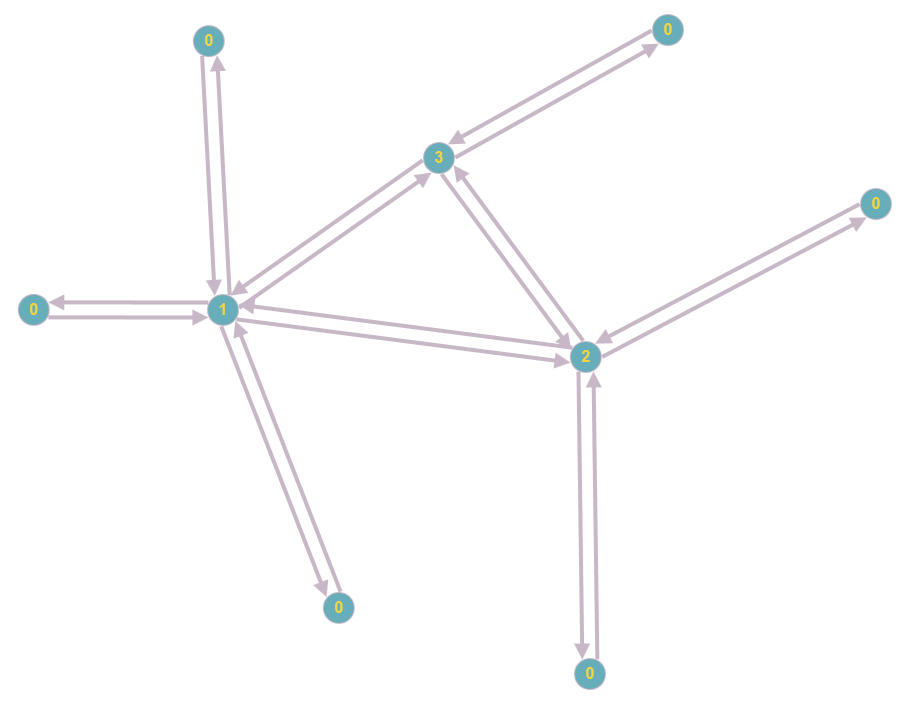
\includegraphics[width=10cm]{network}
%\label{fig:frog1}
%\end{wrapfigure}
%1

\begin{minipage}{12cm}
\begin{figure}[H]
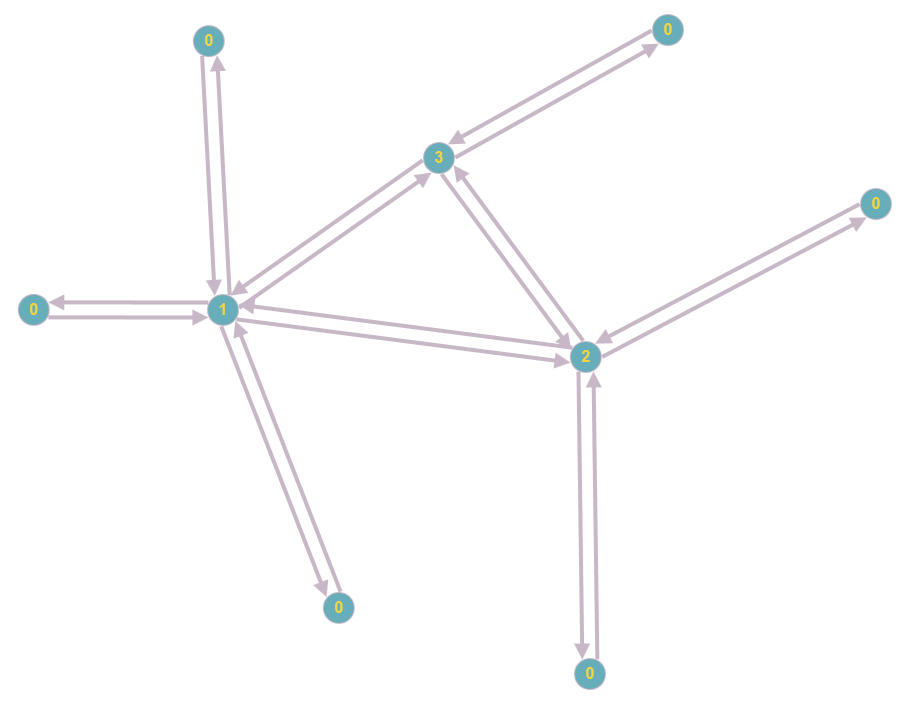
\includegraphics[width=12cm]{network}
\caption{\label{fig:network} Przykładowa sieć dróg}
\end{figure}
\end{minipage} \hfill
\begin{minipage}{5cm}
Skrzyżowania są oznaczone numerami: 1,2,3.
Punkty z numerem 0 są jedynie początkami i końcami dróg.
\end{minipage}
\section{Sygnalizacja świetlna}
Na końcu drogi kończącej się na skrzyżowaniu znajdują się sygnalizacje świetlne, które zezwalają na jazdę w danym kierunku(lub kierunkach). \\
Manewr zdefiniowany jest jako para - kierunku jazdy na skrzyżowaniu (np. w prawo) oraz drogi umożliwiającej wjazd na to skrzyżowanie.\\ Faza świateł to zbiór manewrów, które nie powodują ze sobą kolizji. Tylko jedna faza $M_v$ może być aktywna w danej chwili $t$ i będziemy ją oznaczać z indeksem jako $\overline{M_v}$. Aktywna faza określa zielone światła na sygnalizacjach przypisanych do odpowiadających manewrów fazy.
\newpage
\subsection{Przykład sygnalizacji}
Niech dane będzie skrzyżowanie posiadające po 4 drogi wlotowe i wylotowe. Drogi wlotowe oznaczamy nieparzystymi indeksami jako $E_{in}=\{e^{1},e^{3},e^{5},e^{7}\}$, a wlotowe parzystymi t.j. $E_{in}=\{e^2,e^4,e^6,e^8\}$. Położenie dróg przedstawia rysunek \ref{fig:skrzyzowanie} Każda z dróg wlotowych posiada dwie sygnalizacje świetlne - pierwsza określa możliwość manewru skrętu w lewo, a druga - dwóch manewrów: jazdy prosto i skrętu w prawo. Proponowane fazy to:\\
$M^{(1)}$ - jazda prosto i w prawo dla pasów $e^1$, $ e^5$ \\
$M^{(2)}$ - jazda prosto i w prawo dla pasów $e^3$, $e^7$\\
$M^{(3)}$ - jazda w lewo dla pasów $e^1$, $e^5$\\
$M^{(4)}$ - jazda w lewo dla pasów $e^3$, $e^7$\\
Należy zwrócić uwagę, że jest to tylko jedno z wielu możliwych rozwiązań. Jest ono poprawne, gdyż żadne z manewrów konkretnej fazy się nie wykluczają. Przykładem niepoprawnej fazy jest: \\
$M$ - jazda prosto dla pasów $e^1_{in}$,$e^2_{in}.$Łatwo zauważyć, że te dwa manewry powodują kolizję.
\begin{figure}[H]
  \centering
    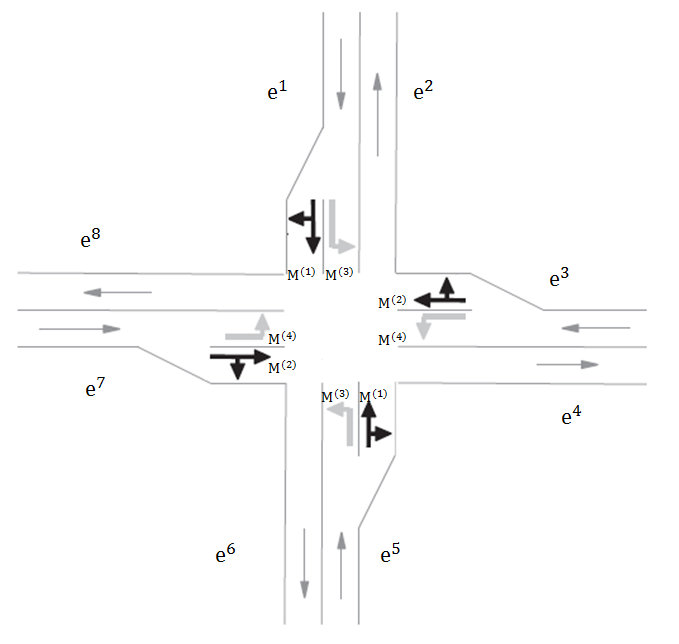
\includegraphics[width=14cm]{skrz_bez_in_out}
 \caption{Skrzyżowanie}
 \label{fig:skrzyzowanie}
\end{figure}

\subsection{Rozkład prawdopodobieństwa manewrów}
Ustalone jest, że wszyscy kierowcy jadący drogą $e$ wjeżdżając na skrzyżowanie $v$ posiadają taki sam rozkład prawdopodobieństwa wyboru kierunku drogi.
Niech manewr  będzie parą $(e,k)$, gdzie $k$ jest kierunkiem obranym na skrzyżowaniu. Prawdopodobieństwo jazdy zgodnie z kierunkiem $k$ oznaczone jest jako  $P_{e,k}$. Aby każdy pojazd opuścił skrzyżowanie funkcja musi spełniać równanie dla dowolnej drogi wlotowej $e$: 
\[
\sum_{k\in K}P_{e,k}=1 \addtag
\]
gdzie $K$ to wszystkie możliwe do wyboru kierunki jazdy na skrzyżowaniu z drogi $e$.

\chapter{Model ruchu drogowego}
\section{Klasyfikacja modeli ruchu drogowego} 
Modele ruchu drogowego mają na celu ukazanie rzeczywistego przepływu pojazdów w sposób czysto matematyczny. Ważnym kryterium doboru modelu jest przystępność jego implementacji informatycznej. Powszechnie klasyfikuje się 3 podejścia modelowe dla omawianego problemu \cite{CompareModels} - makroskopowy, mezoskopowy oraz mikroskopowy. Czasem \cite{multilevel} wyróżnia się także czwarte podejście - submikroskopowe. Jest to podział ze względu na poziom modelu. Najniższy poziom i najbardziej dokładny model gwarantuje podejście mikroskopowe. Rozważa ono pojazdy indywidualnie w czasoprzestrzeni. Przyspieszenie pojazdu jest wyliczane na podstawie dynamiki(prędkości, przyspieszenia) i pozycji pojazdu bezpośrednio przed nim. Model mezoskopowy zapewnia indywidualne rozróżnienie pojazdów, jednak ich zachowanie jest wyliczane na danych zagregowanych \cite{mesoscopic}. Przykładowo pojazdy są zgrupowane w grupę podróżującą z pewnego punktu startowego do celu. Inne modele \cite{mesoscopic2} mezoskopowe wyliczają dynamikę ruchu na podstawie aktualnego zatłoczenia drogi. Poziom mezoskopowy jest obliczeniowo bardziej opłacalny od mikroskopowego.
Wiele symulatorów stosujących model mezoskopowy oferuje symulację w czasie rzeczywistym dla sieci dróg całego miasta\cite{vu2017high}. Ideą modelu makroskopowego jest traktowanie ruchu ulicznego identycznie jak ruchu cieczy lub gazów. Po raz pierwszy w roku 1956 M. J. Lighthill i G. B. Whitham \cite{lwr} przedstawili pomysł przyrównania ruchu ulicznego na zatłoczonych drogach do przepływu wody w rzekach. Z tego powodu nie rozróżniamy w nim indywidualnie pojazdów, ani też nawet grupowo. Rozważamy natomiast gęstość ruchu w danym punkcie na drodze i czasie - czyli ilość pojazdów na danym odcinku drogi. Sposób w jaki poruszają się pojazdy jest wyliczany jedynie na podstawie gęstości ruchu. Jest to najmniej kosztowny obliczeniowo model. Właśnie w modelu makroskopowym zostało stworzone środowisko symulacyjne. Szczegóły modelu są przedstawione w następnym podrozdziale.
\section{Makroskopowy model ruchu} 
\subsection{Wstęp}
Istotą makroskopowego modelu ruchu jest pojęcie gęstości ruchu. Jest to zmienna stanowa określona dla każdego punktu drogi w czasie. Formalnie gęstość można rozumieć jako czynnik definiujący dynamikę ruchu. Im większa gęstość tym mniejsza prędkość ruchu. W niektórych artykułach gęstość ruchu \cite{helbing2001master} jest przedstawiona jako iloraz ilości pojazdów znajdujących się na pewnym odcinku i długości tego odcinka drogi. Nie są to jednak czysto matematyczne formalne definicje. W makroskopowym modelu nie rozróżniamy pojedynczych pojazdów, ani nawet grup, więc taka definicja gęstości ruchu może być odebrana jako nieścisła z ideą modelu. 
\subsection{Rozwój gęstości ruchu na drodze}
Makroskopowy model ruchu jest oparty o równanie różniczkowe (\ref{main_diff_eq}) wraz z warunkiem początkowym (\ref{p_init_eq}) .  Model makroskopowy traktuje ruch uliczny na drogach podobnie do przepływu wody w rzekach. Możemy zatem gęstość ruchu utożsamiać z polem powierzchni przekroju poprzecznego rzeki, co dla ustalonej szerokości rzeki - upraszcza się do wysokości wody w rzece.\\Dla ustalonej drogi $e$ zmianę gęstości ruchu definiuje następujący układ równań:\\
\begin{numcases}{}
   p(x,0)=p_{0}(x) \label{p_init_eq}
   \\
   \frac{\partial p(x,t)}{\partial t}+\frac{\partial f(p(x,t))}{\partial x}=0 \label{main_diff_eq}
\end{numcases}
Gdzie $p(x,t)$ to gęstość ruchu w punkcie $x$ i czasie $t$. Wartość funkcji gęstości należy do przedziału $[0,p^{max}]$.\\
Równanie (\ref{p_init_eq}) zakłada istnienie pewnej z góry nałożonej początkowej gęstości drogi $p_0(x)$.
Równianie (\ref{main_diff_eq}) określa
wedle założeń modelu makroskopowego \cite{lwr} rozwój gęstości ruchu na drodze. Funkcja płynności ruchu $f$ powinna być wklęsła. W przedstawionym w tej pracy modelu funkcja ma następującą definicję:
\begin{numcases}{f(p)=}
   \lambda p & \text{dla } $p\in[0,p^{*}]$\\
   \lambda \cdot (2p^{*}-p) & \text{dla } $p\in(p^{*},p^{max}]$ 
\end{numcases}
Gdzie $\lambda$ jest stałym parametrem funkcji trójkątnej oraz $p^*=\frac{1}{2}p^{max}$.
%\subsection{Rozwój gęstości na skrzyżowaniu}
%Równanie (\ref{main_diff_eq}) dotyczy tylko jednej drogi - nie uwzględnia ono przejazdów na skrzyżowaniu z jednej drogi na drugą. Przedstawiony zatem będzie sposób przepływu ruchu w początkowych ($x=0$) i końcowych ($x=L_e$) punktach drogi $e \in{E}$. 
%Na początku drogi wylotowej $e_{out}$ płynność w dowolnym czasie $t$ wynosi:
%$$\sum_{m_e \in M_e} P_{m_e}f(p(L_e,t)).$$
%Gdzie $M_e$ to zbiór wszystkich manewrów aktywnej fazy świateł, prowadzących do drogi wylotowej $e_{out}$. Gęstości $p(L_e,t)$ odnoszą się do dróg wlotowych $e$. 

%W tym celu ustalmy skrzyżowanie $v$ z drogami wlotowymi $E_{in}$ i wylotowymi $E-{out}$. Zakładamy, że prawdziwa jest równość:
%$$\sum_{{e}\in{E_{in}}} f(p(L_e,t))=\sum_{{e}\in{E_{out}}} f(p(0,t))$$
%Powszechnie stosowane będą następujące oznaczenia gęstości i płynności ruchu dla $x\in(0,L_e)$:
%
%\begin{equation}
%\begin{aligned}
%  p_x^t=p(x,t) \label{p_q_notation}\\
%  q_x^t=q(x,t)
%\end{aligned}
%\end{equation}

%
%Najpierw rozważony zostanie schemat opuszczania drogi przez pojazdy (t.j. wartość $q_{L_e}^t$). Istnieją dwa typy dróg ze względu na ich punkt końcowy. Pierwszy z nich to drogi kończące się na skrzyżowaniu, wtedy ruch przechodzi do dróg wylotowych skrzyżowania. Drugą możliwością jest koniec w punkcie, który jest "krańcem układu". Uznajemy, wtedy, że pojazdy które dotarły do tego punktu skończyły już swoją trasę i przestają istnieć. Zakładamy, że nie ma przeszkód do wjechania do tego punktu i ustalamy końcową płynność jako:
%
%\begin{numcases}{q_{L_e}^t=}
%q(p_v^t) 
% & \text{dla} $p_v^t<\frac{p_{max}}{2}$   \label{q_L_e_normal}
%   \\
%   q(\frac{p_{max}}{2}) & \text{dla} $p_v^t\geq \frac{p_{max}}{2}$   \label{q_L_e_star}
%\end{numcases}
%
%Warto zauważyć, że w przypadku (\ref{q_L_e_star}) duża gęstość (większa od $\frac{p_{max}}{2}$) nie powoduje zmniejszenia płynności tak jak w (\ref{eq:q_pv}). Interpretacja tego faktu jest następująca: pojazdy mogą bezproblemowo opuścić układ - nawet przy dużej gęstości.
%Kolejnym podziałem dróg jest podział ze względu na źródło pojazdów. Pierwszą grupą są drogi posiadające samoistne źródło ruchu w swoim początkowym punkcie. Ruch generowany w tych punktach jest definiowany jako pewna funkcja czasu $q_0^{t}$ o następujących ograniczeniach (todo).
%Kolejną grupą w tym podziale są drogi o punkcie początkowym na skrzyżowaniu $v$. Pojazdy napływające ze skrzyżowania $v$ są wtedy źródłem ruchu. Niech $\overline{M_v^e}$ będzie zbiorem manewrów, które prowadzą do drogi $e$ oraz należą do aktualnie aktywnej fazy $\overline{M_v}$. Wtedy rozważana początkowa płynność to:
%$$q_o^t=\sum_{{m}\in{\overline{M_{v}^{e}}}}P_{m} \cdot q_{L_{e}}^t$$
%Wartość $q$ po prawej stronie równania odnosi się do płynności drogi wlotowej $e$ przyporządkowanej do manewru $w$.

\section{Dyskretyzacja modelu}
Modele dyskretne zazwyczaj są łatwiejsze i mniej kosztowne w implementacji komputerowej. Z tego powodu dokonana zostanie dyskretyzacja osi czasu, modelu sieci drogowej jak i ruchu obowiązującego na niej.
\section{Dyskretyzacja czasu}
Proces dyskretyzacji przeprowadzony zostanie najpierw dla osi czasu. Czas nie będzie traktowany jako wartość ciągła, więc zdefiniujemy przeskok czasu jako $\Delta t$. Przestrzeń czasowa określona jest jako ciąg:
\[
(t_k)_{k=0}^m=k\Delta t \addtag
\]
Gdzie $m$ liczba naturalna określająca moment końca symulacji ruchu drogowego. Oznaczamy go jako $t_{max}=m \cdot \Delta t$.


\section{Dyskretyzacja drogi}
Zadaniem jest określenie ciągu $b_n$ wybranych punktów drogi $e$ dla których będą wyliczane gęstości. Niech dana będzie liczba naturalna $l$ określająca ilość wybranych punktów z drogi. Wtedy odległość między sąsiednimi punktami to $\Delta x=\frac{L_e}{l}$. 
Ciąg $b_n$ jest zdefiniowany następująco: 
\[b_n=n\cdot \Delta x \quad \text{dla }n=0,1,...,l \addtag \label{eq:ciag_bazowy} \]
Powyższy ciąg (\ref{eq:ciag_bazowy}) będzie nazywany siatką bazową. Punkty $b_0$,$b_l$ będziemy dalej nazywać jako punkty brzegowe drogi, a $b_1,...,b_{l-1}$ jako wewnętrzne.\\
Do celów czysto obliczeniowych przedstawionych w rozdziale \ref{sec:dyskretyzacja_ruchu} zostaje utworzona również siatka pomocnicza:
\[\widetilde{b_n}=n\cdot \Delta x+\frac{\Delta x}{2} \quad \text{dla }n=1,...,l \addtag\]

\begin{figure}[H]
  \centering
    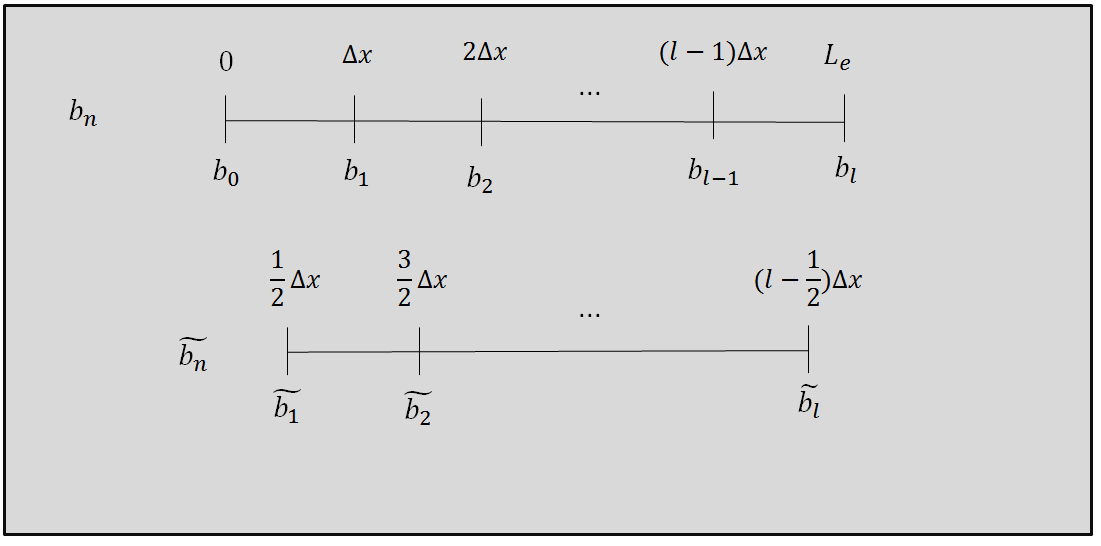
\includegraphics[width=14cm]{odcinki-2}
 \caption{Siatka bazowa $b_n$ i pomocnicza $\widetilde{b_n}$}
 \label{fig:siatka}
\end{figure}
\section{Dyskretyzacja makroskopowego przepływu ruchu}\label{sec:dyskretyzacja_ruchu}
Najpierw rozważone zostaną gęstości ruchu jedynie dla punktów wewnętrznych ciągu $b_n$ czyli z pominięciem $b_0$ i $b_l$.
Dla każdego z tych punktów gęstość będzie wyliczona na podstawie jego otoczenia $(\widetilde{b_{n}},\widetilde{b_{n+1}})$. Gęstość w punkcie $b_n$ i czasie $t_k=k\cdot \Delta t$ definiujemy jako:
\[p_{n}^{k}=\int\limits_{{\widetilde{b_{n}}}}^{{\widetilde{b_{n+1}}}} {\frac{p(x,k \cdot \Delta t)}{\Delta x}dx}. \addtag\]
%Analogicznie definiujemy płynność jako:
%\[q_{n}^{k}=\int\limits_{{\widetilde{b_{n}}}}^{{\widetilde{b_{n+1}}}} {\frac{q(x,k \cdot \Delta t)}{\Delta x}dx}. \addtag \]
 Na podstawie (\ref{main_diff_eq}) możemy wywnioskować, że:
\[\int\limits_{\widetilde{b_{n}}}^{\widetilde{b_{n+1}}} {p(x,t_{k+1})dx-\int\limits_{\widetilde{b_{n}}}^{\widetilde{b_{n+1}}}p(x,t_{k})dx} +\int\limits_{t_k}^{t_{k+1}} q(\widetilde{b_{n+1}},t)-q(\widetilde{b_{n}},t))dt=0 \addtag \label{eq:calki-LWR} \]
Upraszczając otrzymujemy:
\[\Delta x(p_n^{k+1}-p_n^{k}) +\int\limits_{t_k}^{t_{k+1}} q(\widetilde{b_{n+1}},t)-q(\widetilde{b_{n}},t))dt=0 \addtag \]
Przyjmujemy, że wartości przepustowości i gęstości zmieniają się w tylko w chwilach $t_k$. Wtedy wartości $q(\widetilde{b_n},t)$ i $q(\widetilde{b_{n+1}},t)$ są stałe na całym przedziale całkowania $[t_k,t_{k+1})$. Otrzymujemy równanie:
\[\Delta x(p_n^{k+1}-p_n^{k})  + \Delta t (q(\widetilde{b_{n+1}},t_k)-q(\widetilde{b_{n}},t_k))=0 \addtag \]
Rezultatem jest rekurencyjny wzór na gęstość ruchu:
\[p^{k+1}_n=p^{k}_n -\frac{\Delta t}{\Delta x} (q(\widetilde{b_{n+1}},t_k)-q(\widetilde{b_{n}},t_k)) \addtag \label{eq:normal_center_development} \]  
Powyższy wzór zawiera niezdefiniowane wartości $q$ i $p$ dla punktów ciągu $\widetilde{b_n}$ - będziemy je odpowiednio oznaczać $\widetilde{q_{n}^k}$ i $\widetilde{p_{n}^k}$. Dyskretyzacja wedle schematu stagerred Lax-Friedrichs \cite{gottlich} prowadzi do następujących wartości dla dowolnej chwili $t_k$:
\[ 
\widetilde{p_n^k} =  \frac{p_{n-1}^k+p_{n}^k}{2} \addtag \label{eq:init_p_stagerred}
\]
\[ 
\widetilde{q_n^k} =  \frac{q_{n-1}^k+q_{n}^k}{2} \addtag
\]
Ustalona teraz będzie ewolucja gęstości dla pomocniczego ciągu $\widetilde{b_n}$. Jest ona opisana analogicznie do (\ref{eq:normal_center_development}):
\[\widetilde{p^{k+1}_n}=\widetilde{p^k_n}- \frac{\Delta t}{\Delta x}(q(p^k_{n})-q(p^k_{n-1})) \addtag \label{eq:stagered_from_normal} \]
Z równania (\ref{eq:init_p_stagerred}) można wykazać, że dla dowolnego $n$:
\[p_n^{k+1}=\frac{\widetilde{p_{n}^{k+1}}+\widetilde{p_{n+1}^{k+1}}}{2} \addtag
\label{eq:normal_from_stagerred} \]
Na podstawie wzorów (\ref{eq:stagered_from_normal}) i \eqref{eq:normal_from_stagerred} otrzymujemy:
\[ p_n^{k+1} =\frac{1}{2}\widetilde{p^{k}_n}-\frac{\Delta t}{2\Delta x}(q^k_n-q^k_{n-1})+\frac{1}{2}\widetilde{p^{k}_{n+1}}-\frac{\Delta t}{2\Delta x}(q^k_{n+1}-q^k_{n})  \addtag .\]
Co prowadzi do końcowej zależności:
\[ p_n^{k+1} =\frac{1}{2}p_n^k+\frac{1}{4}p_{n+1}^k+\frac{1}{4}p_{n-1}^k  -\frac{\Delta t}{2\Delta x}(q^k_n-q^k_{n-1})-\frac{\Delta t}{2\Delta x}(q^k_{n+1}-q^k_{n}).  \addtag \]


\[ p_n^{k+1} =\frac{1}{2}p_n^k+\frac{1}{4}p_{n+1}^k+\frac{1}{4}p_{n-1}^k  +\frac{\Delta t}{2\Delta x}(q^k_{n-1}-q^k_{n+1})  \addtag \label{eq:final_normal_development}.\]


Powyższy wzór kończy rozważania odnośnie punktów wewnętrznych drogi.
Przypadek punktów brzegowych $b_0,b_l$ różni się diametralnie od punktów wewnętrznych ze względu na to iż trzeba w nich ująć aspekty wprowadzenia nowych pojazdów do ruchu oraz opuszczenia drogi. Podstawowe równanie modelu makroskopowego (\ref{main_diff_eq}) nie uwzględnia ani źródła, ani też ujścia ruchu, co pozwala na zastosowanie własnego rozwiązania w tym zakresie.


\begin{figure}[H]
  \centering
    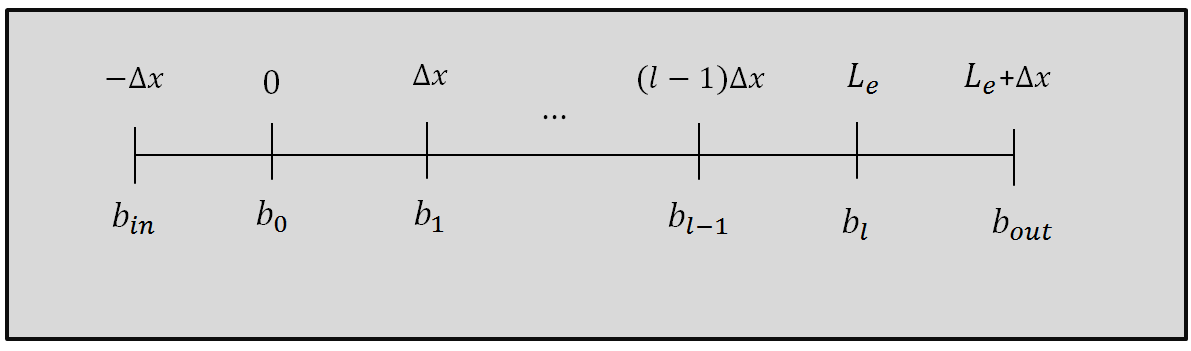
\includegraphics[width=14cm]{odcinki-zrodlo-ujscie}
 \caption{Siatka bazowa $b_n$ wraz ze źródłem i ujściem}
 \label{fig:odcinki-zrodlo-ujscie}
\end{figure}
Przedstawiony w pracy pomysł zakłada, że źródło $b_{in}$ i ujście $b_{out}$ ruchu znajdują się w odległości $\Delta x$ odpowiednio od punktów $b_0$ i $b_l$ (patrz Rysunek \ref{fig:odcinki-zrodlo-ujscie}). \\Gęstość w źródle oznaczamy jako $p^k_{in}$. Rozwój gęstości w początkowym punkcie drogi $b_0$ jest ustalony analogicznym wzorem do (\ref{eq:final_normal_development}):
\[ p_0^{k+1} =\frac{1}{2}p_0^k+\frac{1}{4}p_{1}^k+\frac{1}{4}p^k_{in}  +\frac{\Delta t}{2\Delta x}(q(p^k_{in})-q^k_{1})  \addtag .\]
Gęstość ujścia oznaczona jest jako $p^k_{out}$. Gęstość w końcowym punkcie drogi $b_l$ cechuje się następującą zmiennością:
\[ p_l^{k+1} =\frac{1}{2}p_l^k+\frac{1}{4}p^k_{out}+\frac{1}{4}p^k_{l-1}  +\frac{\Delta t}{2\Delta x}(q(p^k_{l-1})-q(p^k_{out}))  \addtag .\]
W przypadku pojedynczej drogi $p_0^k$ może być dowolną funkcją. Z kolei $p_l^k$ zakładając, że pojazdy nie mają problemu z opuszczeniem drogi jest równe 0. 
\section{Przepływ ruchu na skrzyżowaniu 1}
Udało się przedstawić przepływ ruchu dla pojedynczej drogi. W tym momencie należy skonstruować logiczny model przepływu ruchu przez skrzyżowanie. Początkowo wykorzystany będzie bardzo prosty przykład, aby ustalić przepływ ruchu na skrzyżowaniu. Skrzyżowanie jest przedstawione na rysunku \ref{fig:skrz_1}.
\begin{figure}[H]
  \centering
    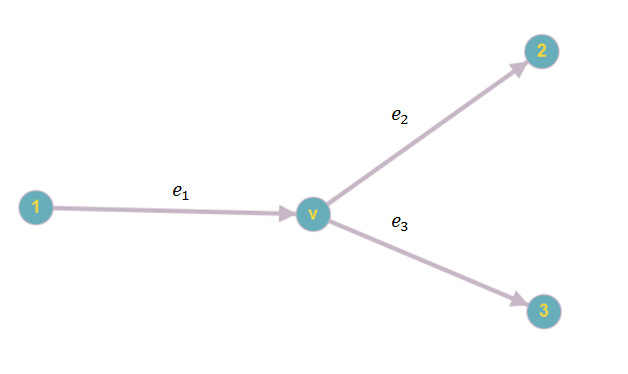
\includegraphics[width=14cm]{skrz_1}
 \caption{Skrzyzowanie 1}
 \label{fig:skrz_1}
\end{figure}
Skrzyżowanie $v$ posiada dwie drogi wlotowe $e_1,e_2$ oraz jedną wylotową $e_3$. Źródła ruchu dla tej sieci dróg znajdują się na początku dróg $e_1,e_2$ (punkty 1 i 2 na Rysunku \ref{fig:skrz_1}). Należy podkreślić, że ujścia dróg $e_1,e_2$ i źródło drogi $e_3$ są fizycznie w tym samym punkcie oznaczonym jako $v$. Gęstość w tym punkcie w chwili $t_k$ będziemy oznaczać jako $p_v^k$.\\
Skrzyżowanie posiada dwie fazy świateł:\\
$M^{(1)}$ - umożliwiające jazdę w lewo z drogi $e_1$\\
$M^{(2)}$ - umożliwiające jazdę w prawo z drogi $e_2$ \\
Bazując na wzorach opisujących rozwój gęstości w dyskretnym modelu   przedstawiony zostanie wzór opisujący rozwój gęstości w punkcie $v$.

\begin{numcases}{p_{v}^{k+1}=}
    \frac{1}{2}p_v^k+\frac{1}{4} {_3p_{0}^k}+\frac{1}{4}{_1p_{out}^k}   +\frac{\Delta t}{2\Delta x}({_1q^k_{out}}-{_3q^k_{0}}) & \text{gdy } $M^{(1)}$ jest aktywną fazą\\
   \frac{1}{2}p_v^k+\frac{1}{4} {_3p_{0}^k}+\frac{1}{4}{_2p_{out}^k}   +\frac{\Delta t}{2\Delta x}({_2q^k_{out}}-{_3q^k_{0}}) & \text{gdy } $M^{(2)}$ jest aktywną fazą 
\end{numcases}
Szczegółowa dane pozwalające na przeprowadzenie symulacji są następujące: \\
$_1p_{in}^k=0.2$ \\
$_2p_{in}^k=0.1$ \\
$p_{max}=0.25$ (dla wszystkich dróg)\\
$\Delta x=50$\\
$\Delta t=1$ \\
$\lambda=2$ \\
$L_{e_1},L_{e_2},L_{e_3}=200$
\begin{figure}[H]
  \centering
    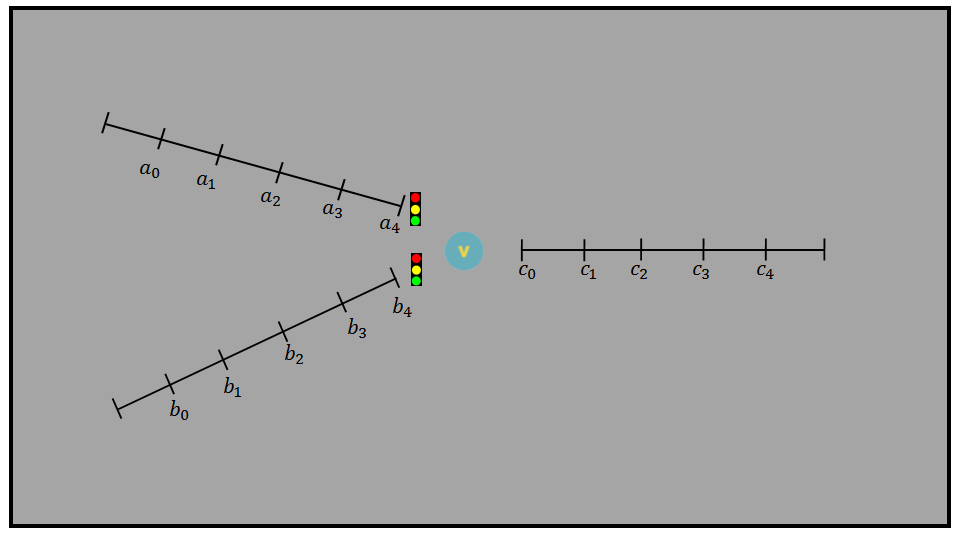
\includegraphics[width=14cm]{skrz_1_discret}
 \caption{Skrzyzowanie 1}
 \label{fig:skrz_1}
\end{figure}

%\\Uznajemy, że na początku symulacji ruchu nie ma żadnych pojazdów co jest równoważne z zerową gęstością ruchu. \\Źródła ruchu znajdują się na początku dróg $e_1,e_2$ (punkty 1 i 2). 
%Ustalamy, że źródła mają stałą w czasie gęstość ruchu 0.1. \\Wszystkie 3 drogi mają $p_{max}=1$. 




\bibliographystyle{IEEEtran}
\bibliography{refs}
\end{document}
